\chapter{Conclusion et perspectives}
\renewcommand\chapterillustration{CON/CON}
\ThisULCornerWallPaper{1}{\chapterillustration}
%\minitoc
\vspace*{-0.5cm}
\lettrine[lines=4, slope=-0.5em,nindent=10pt]{A}{vec} la mise à niveau du LHC en HL-LHC prévue pour \num{2026}, la luminosité instantanée et le pile-up des événements vont augmenter de façon significative. Afin de faire face à cette augmentation du taux de collisions, le détecteur CMS doit être lui aussi mis à niveau. De nombreux changements dans presque tous ses sous-détecteurs sont prévus.

Dans le trajectographe à muons, et notamment dans les bouchons, le programme d'amélioration prévoit, entre autres, d'instrumenter les zones RE3/1 et RE4/1 avec des RPC de nouvelle génération appelées iRPC. Ces zones initialement prévues pour être instrumentées par des RPC dès le début de la construction de CMS en sont toujours dépourvues en raison du flux important de particules les traversant.

Fort des connaissances et de l'expertise acquises sur les GRPC, depuis plus de dix ans, lors de la construction du SDHCAL pour ILC, l'IPNL a décidé de s'investir dans la mise à niveau des bouchons de CMS. Une collaboration avec nos collègues chinois de Tsinghua a permis de proposer l'utilisation de verre de basse résistivité \SI{e10}{\ohm\centi\meter} comme électrodes pour les chambres RPC dans les zones à instrumenter RE3/1 ET RE4/1. 

Cette thèse a eu pour but de caractériser ces verres et de vérifier s'ils pouvaient être utilisés pour la construction de chambres RPC en vue de l'instrumentation de ces zones. Pour cela, de nombreux tests en faisceaux au PS, SPS, et GIF++ ont été réalisés. Ces tests ont montré que ce type de verres pouvait résister à des flux de particules très importants pour des RPC : \SI{3}{\kilo\hertz\per\square\centi\meter}. Nous avons également démontré qu'il était possible de construire des chambres de grande taille (RE1/1) avec ces verres, limités par leur procédé de fabrication à une surface de \SI{32}{\centi\meter}$\times$\SI{30}{\centi\meter}. Cependant, ces verres semblent inadaptés au mélange de gaz utilisé dans CMS. Des tests effectués à Lyon et au CERN tendent à démontrer que ce type de verre nécessiterait un mélange gazeux comportant une proportion plus importante de \chemform{SF_6} que celle utilisée dans CMS afin de réduire significativement le bruit. De plus, étant donné les problèmes rencontrés sur notre installation au GIF++, nous n'avons pas été en mesure de démontrer que ces verres résisteront à \num{10} ans d'opération de CMS.

Parallèlement, nous avons proposé un nouveau type de PCB basé sur des ASIC PETIROC2 et permettant de lire les strips des chambres des deux côtés. Ce type de lecture permet de supprimer le partitionnement et permet également d'obtenir la position du hit le long des strips. Des tests effectués en mai \num{2017} sur la ligne H4 ont ainsi montré que cette position pouvait être connue avec une résolution de l'ordre de \SI{1.8}{\centi\meter} contre une résolution correspondant à la longueur des strips actuellement. Ces résultats, très satisfaisants, malgré certains problèmes sur le PCB et l'absence de calibration des strips ont amené la communauté muons de CMS à choisir cette méthode de lecture comme solution privilégiée pour le TDR actuellement en cours de rédaction.

De nombreuses améliorations et adaptations de cette électronique sont dès à présent prévu. La valeur minimale de la gamme dynamique du seuil va être baissée afin de déclencher sur des signaux de \SI{10}{\femto\coulomb}, la technologie \chemform{SiGe} à \SI{350}{\nano\meter} va être remplacée par une technologie CMOS à \SI{130}{\nano\meter} par l'entreprise \textit{Taiwan Semiconductor Manufacturing Company} (TSMC) afin de rendre cet ASIC plus tolérant aux radiations. Son nombre de voies d'entrées va également être augmenté et passer de \num{32} à \num{64}.

Les mezzanines contenant les TDC vont être remplacées par des FPGA. Une alternative permettant d'intégrer les TDC directement dans les ASIC est également à l'étude. Cette solution, présente l'avantage de diminuer la consommation électrique et évite les problèmes de routage des données; elle reposera sur des TDC utilisant le principe de Vernier (cf.Fig~\ref{vernier}). Ce type de TDC utilise deux oscillateurs de fréquences très proches l'une de l'autre afin de mesurer le temps.

\begin{figure}[ht!]
	\centering
	\subfloat[Schèma de principe du TDC de type Vernier.]{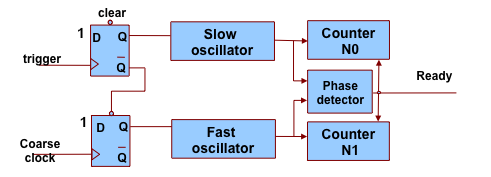
\includegraphics[width=0.49\textwidth]{CON/Vernier1.png}}
	\hfill
	\subfloat[Diagramme temporelle du principe de Vernier.]{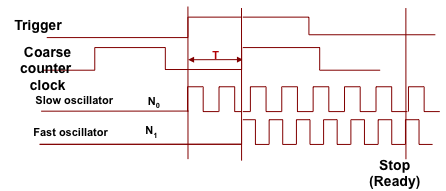
\includegraphics[width=0.49\textwidth]{CON/Vernier2.png}}
	\caption{Schéma de principe et diagramme temporel du principe des TDC utilisant le principe de Vernier. Le temps calculé par le TDC est donné par $T=N_0T_{slow}-N_1T_{fast}$ avec $N_0$ ($N_1$) le nombre d'oscillations de l'oscillateur lent (rapide).}
	\label{vernier}
\end{figure}

Toute cette électronique est placée sur une mezzanine fixée directement sur les chambres (cf.Fig~\ref{chamber}). Des câbles coaxiaux sont soudés à l'extremité des strips d'un côté et sont reliés de l'autre à une carte, raccordée à la mezzanine qui permet, pour chaque câble d'adapter l'impédance à celle des voies d'entrée des ASIC ($\sim$\SI{200}{\ohm}).  

\begin{figure}[ht!]
	\centering
	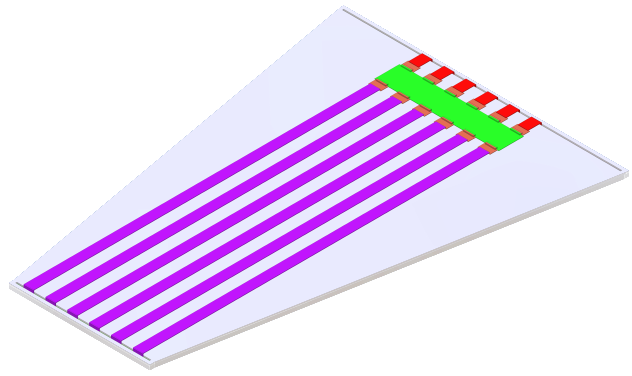
\includegraphics[width=0.50\textwidth]{CON/chambre.png}
	\captionof{figure}{Schéma d'une chambre iRPC avec l'électronique PETIROC2. La mezzanine est en vert. Les câbles coaxiaux venant des deux côtés des strips ( en violet et en rouge) sont connectés à la mezzanine par des cartes adaptatrices d'impédance (en orange). Le détecteur et le PCB avec les strips sont à l'intérieur de la mécanique et ne sont pas visibles.}
	\label{chamber}
\end{figure}

Les mezzanines seront reliées à la DAQ par des \textit{Low power GigaBit Transceiver} (LpGBT) qui assureront également la connexion entre les ASIC et les TDC (cf.Fig~\ref{chambres}). 

\begin{figure}[ht!]
	\centering
	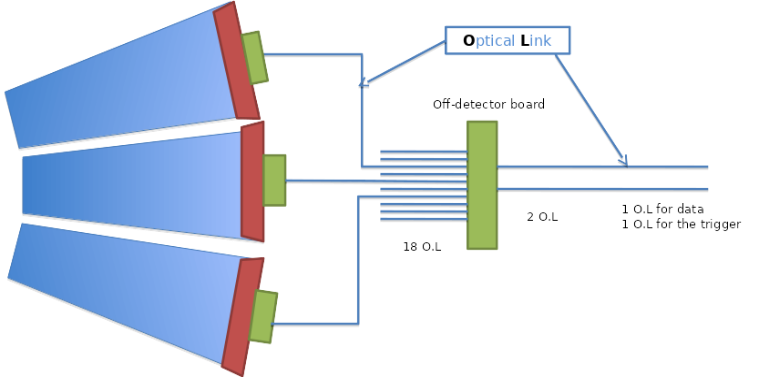
\includegraphics[width=0.70\textwidth]{CON/chambres.png}
	\captionof{figure}{Schéma du système DAQ des nouvelles chambres.}
	\label{chambres}
\end{figure}

Des prototypes de PCB comportant \num{96} strips et faisant la taille d'une demi chambre RE3/1 en $\phi$ \footnote{Ceci est nécessaire car la fabrication de PCB de grande taille est aujourd'hui très compliquée.} (cf.Fig~\ref{proto}) ont été fabriqués et sont en phase de test à Lyon. Un autre type incorporant les retours des strips directement dans le PCB et ne nécessitant donc pas de souder des câbles coaxiaux aux strips est également à l'étude.

\begin{figure}[ht!]
	\centering
	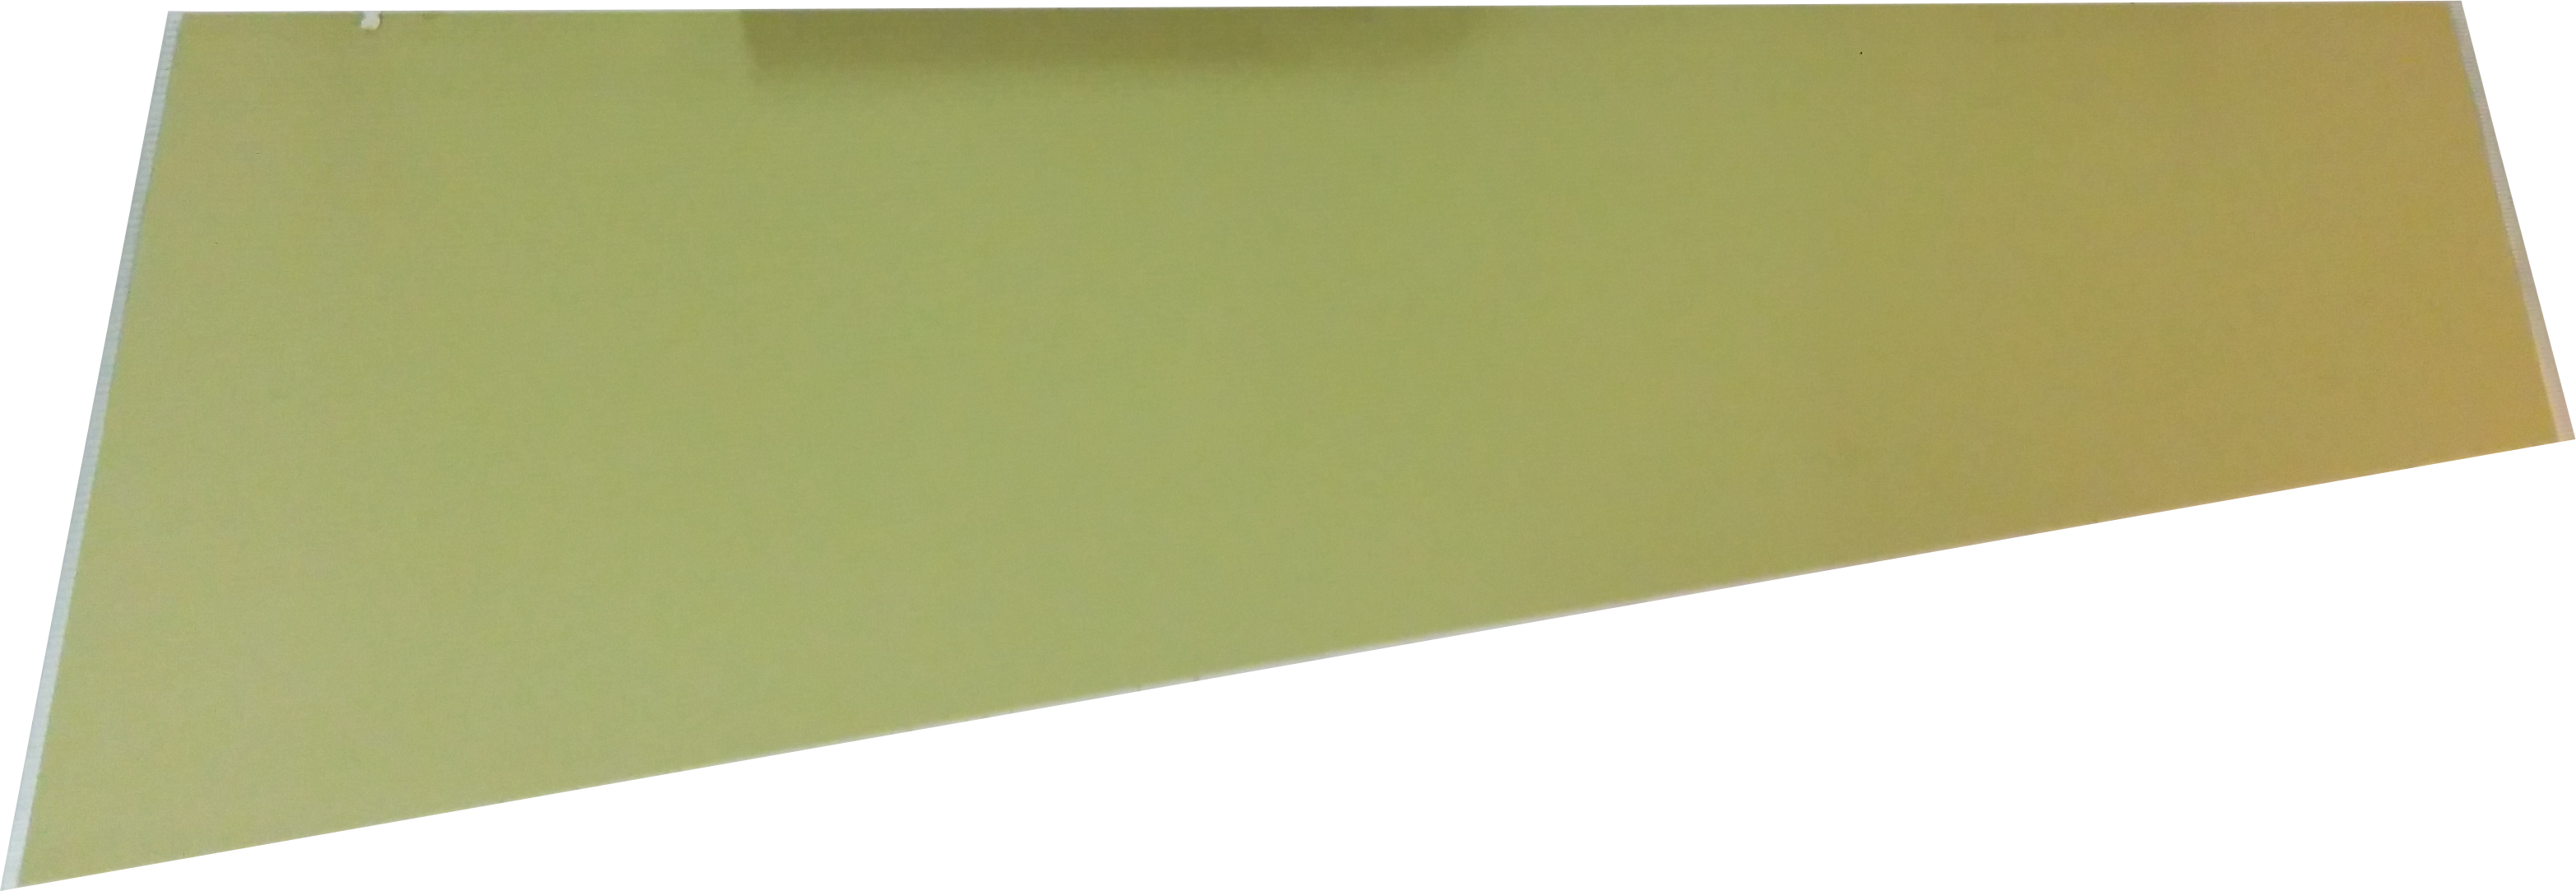
\includegraphics[width=0.75\textwidth]{CON/proto.png}
	\captionof{figure}{Le prototype de PCB avec lecture des strips des deux côtés.}
	\label{proto}
\end{figure}